%%%%%%%%%%%%%%%%%%%%%%%%%%%%%%%%%%%%%%%%%
% Programming/Coding Assignment
% LaTeX Template
%
% This template has been downloaded from:
% http://www.latextemplates.com
%
% Original author:
% Ted Pavlic (http://www.tedpavlic.com)
%
% Note:
% The \lipsum[#] commands throughout this template generate dummy text
% to fill the template out. These commands should all be removed when 
% writing assignment content.
%
% This template uses a Perl script as an example snippet of code, most other
% languages are also usable. Configure them in the "CODE INCLUSION 
% CONFIGURATION" section.
%
%%%%%%%%%%%%%%%%%%%%%%%%%%%%%%%%%%%%%%%%%

%----------------------------------------------------------------------------------------
%	PACKAGES AND OTHER DOCUMENT CONFIGURATIONS
%----------------------------------------------------------------------------------------

\documentclass{article}

\usepackage{fancyhdr} % Required for custom headers
\usepackage{lastpage} % Required to determine the last page for the footer
\usepackage{extramarks} % Required for headers and footers
\usepackage[usenames,dvipsnames]{color} % Required for custom colors
\usepackage{graphicx} % Required to insert images
\usepackage{listings} % Required for insertion of code
\usepackage{courier} % Required for the courier font
\usepackage{lipsum} % Used for inserting dummy 'Lorem ipsum' text into the template

\usepackage{enumerate}
\usepackage{amsmath}
\usepackage{hyperref}

\usepackage{graphicx}
\usepackage{caption}
\usepackage{subcaption}

\usepackage{listings}
\usepackage{color} %red, green, blue, yellow, cyan, magenta, black, white
\usepackage{gensymb}

\definecolor{mygreen}{RGB}{28,172,0} % color values Red, Green, Blue
\definecolor{mylilas}{RGB}{170,55,241}

% Margins
\topmargin=-0.45in
\evensidemargin=0in
\oddsidemargin=0in
\textwidth=6.5in
\textheight=9.0in
\headsep=0.25in

\linespread{1.1} % Line spacing

% Set up the header and footer
\pagestyle{fancy}
\lhead{\hmwkAuthorName} % Top left header
\chead{\hmwkClass\ (\hmwkClassInstructor\ \hmwkClassTime): \hmwkTitle} % Top center head
\rhead{\firstxmark} % Top right header
\lfoot{\lastxmark} % Bottom left footer
\cfoot{} % Bottom center footer
\rfoot{Page\ \thepage\ of\ \protect\pageref{LastPage}} % Bottom right footer
\renewcommand\headrulewidth{0.4pt} % Size of the header rule
\renewcommand\footrulewidth{0.4pt} % Size of the footer rule

\setlength\parindent{0pt} % Removes all indentation from paragraphs

%----------------------------------------------------------------------------------------
%	CODE INCLUSION CONFIGURATION
%----------------------------------------------------------------------------------------

\definecolor{MyDarkGreen}{rgb}{0.0,0.4,0.0} % This is the color used for comments
\lstloadlanguages{Perl} % Load Perl syntax for listings, for a list of other languages supported see: ftp://ftp.tex.ac.uk/tex-archive/macros/latex/contrib/listings/listings.pdf
\lstset{language=Perl, % Use Perl in this example
        frame=single, % Single frame around code
        basicstyle=\small\ttfamily, % Use small true type font
        keywordstyle=[1]\color{Blue}\bf, % Perl functions bold and blue
        keywordstyle=[2]\color{Purple}, % Perl function arguments purple
        keywordstyle=[3]\color{Blue}\underbar, % Custom functions underlined and blue
        identifierstyle=, % Nothing special about identifiers                                         
        commentstyle=\usefont{T1}{pcr}{m}{sl}\color{MyDarkGreen}\small, % Comments small dark green courier font
        stringstyle=\color{Purple}, % Strings are purple
        showstringspaces=false, % Don't put marks in string spaces
        tabsize=5, % 5 spaces per tab
        %
        % Put standard Perl functions not included in the default language here
        morekeywords={rand},
        %
        % Put Perl function parameters here
        morekeywords=[2]{on, off, interp},
        %
        % Put user defined functions here
        morekeywords=[3]{test},
       	%
        morecomment=[l][\color{Blue}]{...}, % Line continuation (...) like blue comment
        numbers=left, % Line numbers on left
        firstnumber=1, % Line numbers start with line 1
        numberstyle=\tiny\color{Blue}, % Line numbers are blue and small
        stepnumber=5 % Line numbers go in steps of 5
}

% Creates a new command to include a perl script, the first parameter is the filename of the script (without .pl), the second parameter is the caption
\newcommand{\perlscript}[2]{
\begin{itemize}
\item[]\lstinputlisting[caption=#2,label=#1]{#1.pl}
\end{itemize}
}

%----------------------------------------------------------------------------------------
%	DOCUMENT STRUCTURE COMMANDS
%	Skip this unless you know what you're doing
%----------------------------------------------------------------------------------------

% Header and footer for when a page split occurs within a problem environment
\newcommand{\enterProblemHeader}[1]{
\nobreak\extramarks{#1}{#1 continued on next page\ldots}\nobreak
\nobreak\extramarks{#1 (continued)}{#1 continued on next page\ldots}\nobreak
}

% Header and footer for when a page split occurs between problem environments
\newcommand{\exitProblemHeader}[1]{
\nobreak\extramarks{#1 (continued)}{#1 continued on next page\ldots}\nobreak
\nobreak\extramarks{#1}{}\nobreak
}

\setcounter{secnumdepth}{0} % Removes default section numbers
\newcounter{homeworkProblemCounter} % Creates a counter to keep track of the number of problems

\newcommand{\homeworkProblemName}{}
\newenvironment{homeworkProblem}[1][Problem \arabic{homeworkProblemCounter}]{ % Makes a new environment called homeworkProblem which takes 1 argument (custom name) but the default is "Problem #"
\stepcounter{homeworkProblemCounter} % Increase counter for number of problems
\renewcommand{\homeworkProblemName}{#1} % Assign \homeworkProblemName the name of the problem
\section{\homeworkProblemName} % Make a section in the document with the custom problem count
\enterProblemHeader{\homeworkProblemName} % Header and footer within the environment
}{
\exitProblemHeader{\homeworkProblemName} % Header and footer after the environment
}

\newcommand{\problemAnswer}[1]{ % Defines the problem answer command with the content as the only argument
\noindent\framebox[\columnwidth][c]{\begin{minipage}{0.98\columnwidth}#1\end{minipage}} % Makes the box around the problem answer and puts the content inside
}

\newcommand{\homeworkSectionName}{}
\newenvironment{homeworkSection}[1]{ % New environment for sections within homework problems, takes 1 argument - the name of the section
\renewcommand{\homeworkSectionName}{#1} % Assign \homeworkSectionName to the name of the section from the environment argument
\subsection{\homeworkSectionName} % Make a subsection with the custom name of the subsection
\enterProblemHeader{\homeworkProblemName\ [\homeworkSectionName]} % Header and footer within the environment
}{
\enterProblemHeader{\homeworkProblemName} % Header and footer after the environment
}

%----------------------------------------------------------------------------------------
%	NAME AND CLASS SECTION
%----------------------------------------------------------------------------------------

\newcommand{\hmwkTitle}{Homework\ \#7} % Assignment title
\newcommand{\hmwkDueDate}{Tuesday,\ October\ 27,\ 2015} % Due date
\newcommand{\hmwkClass}{CSC 514: Computer Vision} % Course/class
\newcommand{\hmwkClassTime}{11:00am} % Class/lecture time
\newcommand{\hmwkClassInstructor}{Hoover} % Teacher/lecturer
\newcommand{\hmwkAuthorName}{Julian A. Brackins} % Your name

%----------------------------------------------------------------------------------------
%	TITLE PAGE
%----------------------------------------------------------------------------------------

\title{
\vspace{2in}
\textmd{\textbf{\hmwkClass:\ \hmwkTitle}}\\
\normalsize\vspace{0.1in}\small{Due\ on\ \hmwkDueDate}\\
\vspace{0.1in}\large{\textit{\hmwkClassInstructor\ \hmwkClassTime}}
\vspace{3in}
}

\author{\textbf{\hmwkAuthorName}}
\date{} % Insert date here if you want it to appear below your name

%----------------------------------------------------------------------------------------

\begin{document}

\maketitle

%----------------------------------------------------------------------------------------
%	TABLE OF CONTENTS
%----------------------------------------------------------------------------------------

%\setcounter{tocdepth}{1} % Uncomment this line if you don't want subsections listed in the ToC

\newpage

\newpage

%----------------------------------------------------------------------------------------
%	PROBLEM 1
%----------------------------------------------------------------------------------------

% To have just one problem per page, simply put a \clearpage after each problem

\begin{homeworkProblem}
Using your functions developed in Homework 6 to computer convolution and correlation of images
with a specified kernel, in this homework you will develop a function to compute the edges of an input
image. Your function will take as input an image and a kernel and output an edge map of the input
image. You may want to create a second function to return the kernel based on use input (i.e., Roberts,
Sobel, Prewet, and Gaussian). In addition, you will want your output image to be the same size as the
input image, therefore, you'll need to deal with the edges accordingly and document in your write-up.

\section{Preface}
In the previous program, we examined how using correlation could be utilized to find similarities between an image and a kernel. In this assignment, convolution is used to find differences between images and a kernel. These differences in images can be used to generate what is known as an edge map. Edges arise from various reasons in images. Edges can be seen in changes of reflectance or texture, changes in surface orientation, or even in cast shadows. In a perfect world, edges are used to determine depth discontinuity and identify object boundaries. 

\section{Equations}
This assignment once again utilizes the Convolution equation. \\ \\

\textbf{Convolution:} $$G\Big[ i , j \Big] = \sum\limits_{u=-k}^{k} \sum\limits_{v=-k}^{k} H\Big[ u , v \Big]F\Big[ i - u , j - v \Big]$$ \\

Where $F$ is the image and $H$ is the kernel. \\ 
Convolution can actually be performed using Correlation. Flip the kernel in both directions (or rotate the kernel 180\degree), then apply correlation. \\


In this assignment, finite difference kernels are also utilized. The following family of gradient kernels, also known as a mask, will be used for this program:

 $$G_{x} = 
 \begin{bmatrix}
-1 & 0 & 1 \\
2 - p & 0 & p - 2 \\
-1 & 0 & 1 \\
\end{bmatrix}$$

 $$G_{y} = 
 \begin{bmatrix}
-1 & 2 - p & -1 \\
0 & 0 & 0 \\
1 & p - 2 & 1 \\
\end{bmatrix}$$

Where $p$ varies based on the type of kernel being used:

$$
\begin{tabular}{ | l | c | c | r |}
   \hline
   & Prewitt & Sobel & Isotropic \\
  \hline
  \hline
  $p$ & $3$ & $4$ & $2 + \sqrt{2}$  \\
  \hline

\end{tabular}
$$ \\


Finally, in order to generate the edge map, the gradient magnitude formula will be used.

$$
   \mid \mid \bigtriangledown f \mid \mid = \sqrt{ (\frac{\delta f}{\delta x})^{2} + (\frac{\delta f}{\delta y})^{2} }
$$ 

Where $\frac{\delta f}{\delta x})$ is the $x$ derivative map generated from the  $G_{x}$ gradient, and  $\frac{\delta f}{\delta y})$ is the $y$ derivative map generated from the  $G_{y}$ gradient.

\section{Process}

The following is the process used to find the edges.
\begin{itemize}
	\item Read in the image.
	\item Convert image to grayscale double.
	\item Determine kernel used for edge detection (Roberts, Sobel, Prewitt, or Gaussian)
	\item Calculate x derivative and y derivative from kernels using Convolution:
	\begin{itemize}
		\item Rotate kernel by 180 degrees.
		\item Pad image edges to retain appropriate dimensions (see Image Padding subsection)
		\item Perform Correlation
	\end{itemize}
	\item Generate Edge Map by using gradient magnitude.
\end{itemize}

\subsection{Image Padding}
Image padding is required for applying the kernel to the input image. In order to do this, we'll use the functions $vertcat()$ and $horzcat()$. The $vertcat()$ method will put horizontal bars on the top and bottom of the image, and $horzcat()$ will put vertical bars on the left and the right of the image. The kernel size is used to determine the size of the horizontal and vertical bars that are added to the image. Refer to Line 15 in Listing 5 (the Convolution function) for a representation of how $horzcat()$ and $vertcat()$ are utilized to add the padding.


\section{Matlab}
The Matlab Code for the program attached after the conclusion of this Homework Document.

\section{Conclusion}
This assignment covers the utility of convolution in detecting edges in images. The real-world applications of this skill are wide spread. In computer vision, the ability to discern edges in a scene can allow a computer to have a better spacial understanding of a given area. The different kernels used to create the edge maps are shown on the following pages, as well as the x and y derivative images.



\begin{figure}[h]
	\centering
	\begin{subfigure}{.5\textwidth}
		  \centering
		  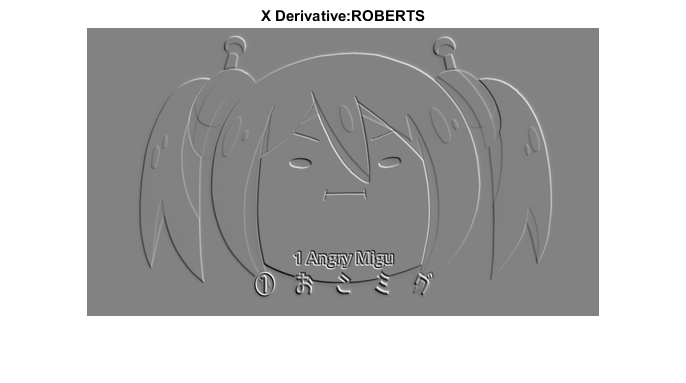
\includegraphics[width=1\linewidth]{img/rob1x}
		  \caption{X Derivative}
		  \label{fig:robX}
	\end{subfigure}%
	\begin{subfigure}{.5\textwidth}
		  \centering
		  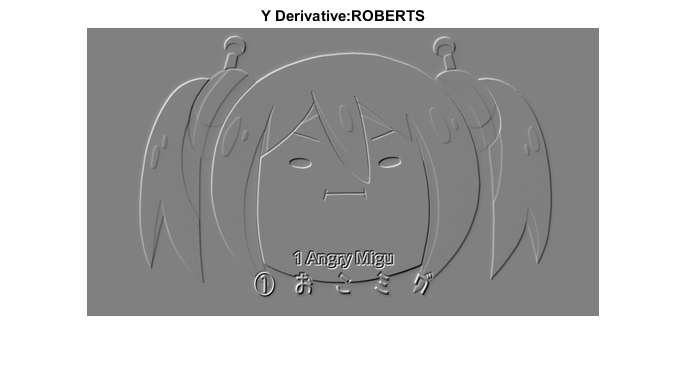
\includegraphics[width=1\linewidth]{img/rob2y}
		  \caption{Y Derivative}
		  \label{fig:robY}
	\end{subfigure}
	\caption{Derivative Maps Using Roberts}
	\label{fig:rob1}
\end{figure}

\begin{figure}[h]
	\centering
	\begin{subfigure}{.5\textwidth}
		  \centering
		  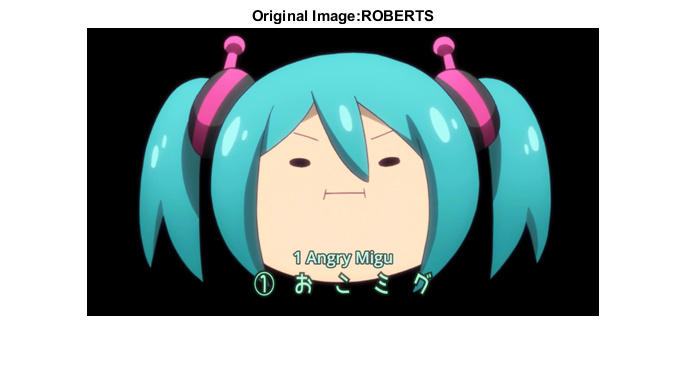
\includegraphics[width=1\linewidth]{img/rob0orig}
		  \caption{Original Image}
		  \label{fig:robOrig}
	\end{subfigure}%
	\begin{subfigure}{.5\textwidth}
		  \centering
		  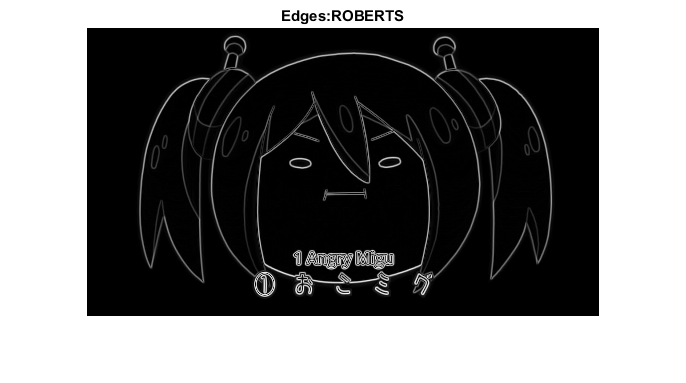
\includegraphics[width=1\linewidth]{img/rob3edge}
		  \caption{Edge Map}
		  \label{fig:robEdge}
	\end{subfigure}
	\caption{Edge Detection Using Roberts}
	\label{fig:rob2}
\end{figure}


%%%%%%%%%%%%%%%%%%%%%%




\begin{figure}[h]
	\centering
	\begin{subfigure}{.5\textwidth}
		  \centering
		  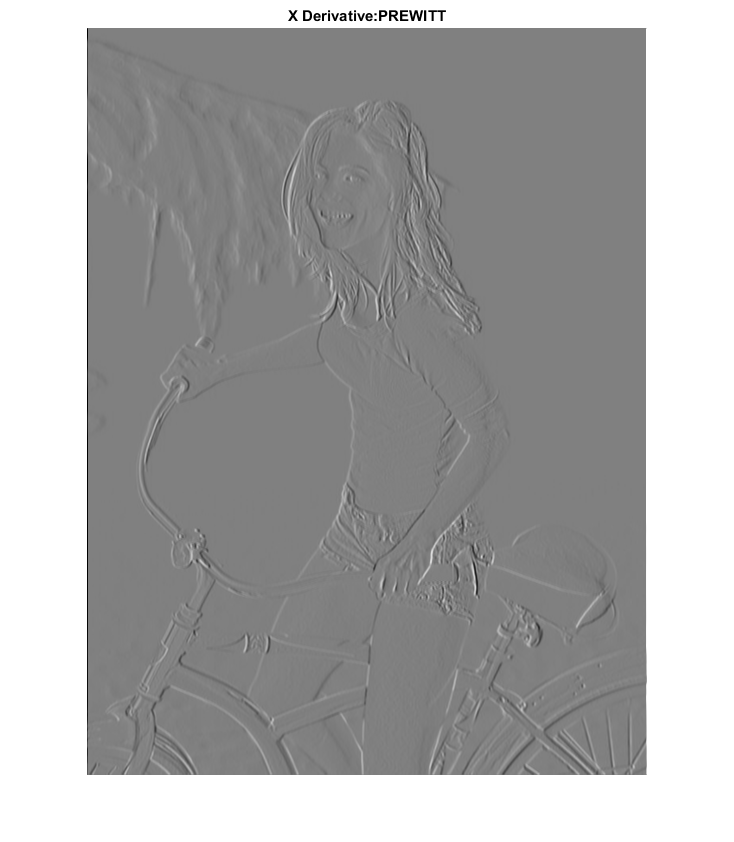
\includegraphics[width=1\linewidth]{img/pre1x}
		  \caption{X Derivative}
		  \label{fig:preX}
	\end{subfigure}%
	\begin{subfigure}{.5\textwidth}
		  \centering
		  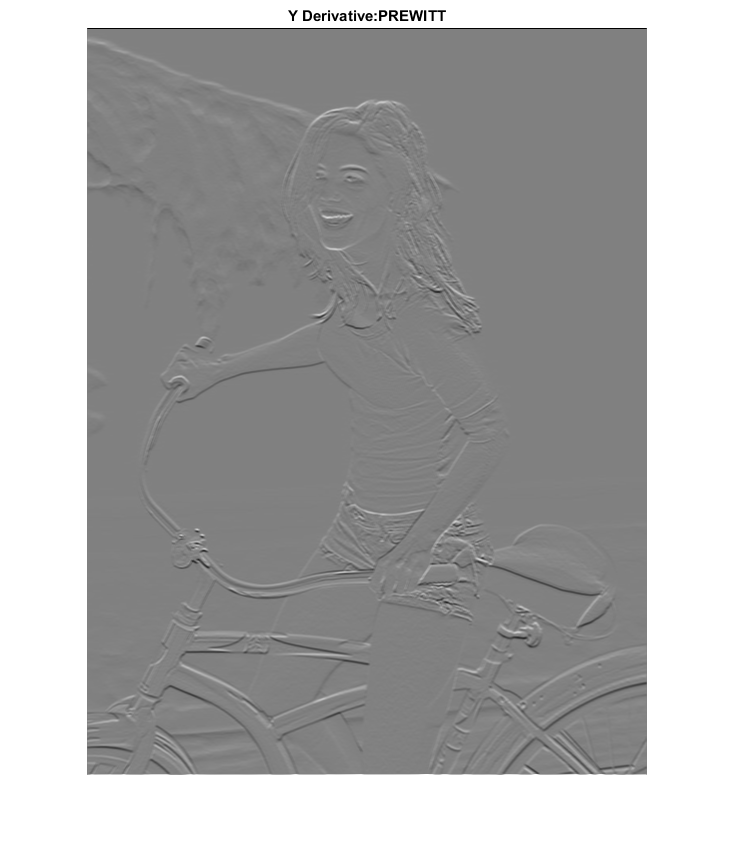
\includegraphics[width=1\linewidth]{img/pre2y}
		  \caption{Y Derivative}
		  \label{fig:preY}
	\end{subfigure}
	\caption{Derivative Maps Using Prewitt}
	\label{fig:pre1}
\end{figure}

\begin{figure}[h]
	\centering
	\begin{subfigure}{.5\textwidth}
		  \centering
		  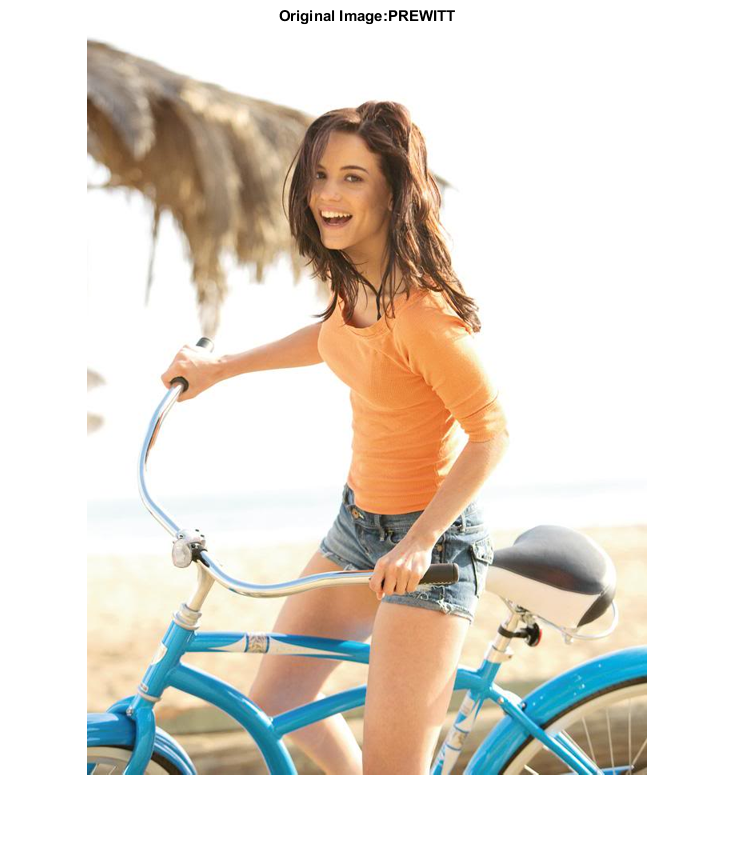
\includegraphics[width=1\linewidth]{img/pre0orig}
		  \caption{Original Image}
		  \label{fig:preOrig}
	\end{subfigure}%
	\begin{subfigure}{.5\textwidth}
		  \centering
		  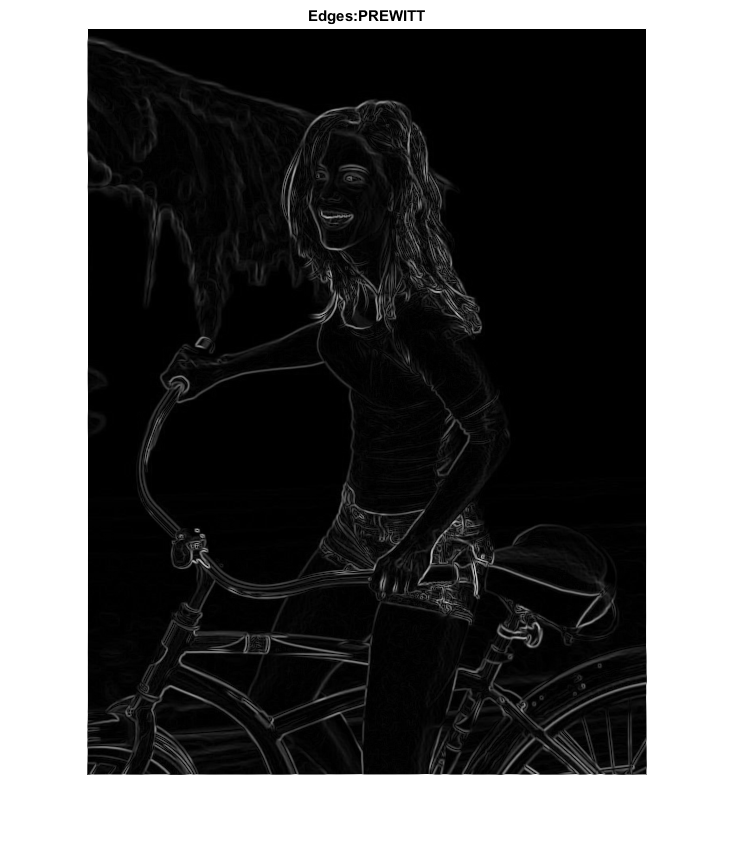
\includegraphics[width=1\linewidth]{img/pre3edge}
		  \caption{Edge Map}
		  \label{fig:preEdge}
	\end{subfigure}
	\caption{Edge Detection Using Prewitt}
	\label{fig:pre2}
\end{figure}

%%%%%%%%%%%%%%%%%%%%%%




\begin{figure}[h]
	\centering
	\begin{subfigure}{.5\textwidth}
		  \centering
		  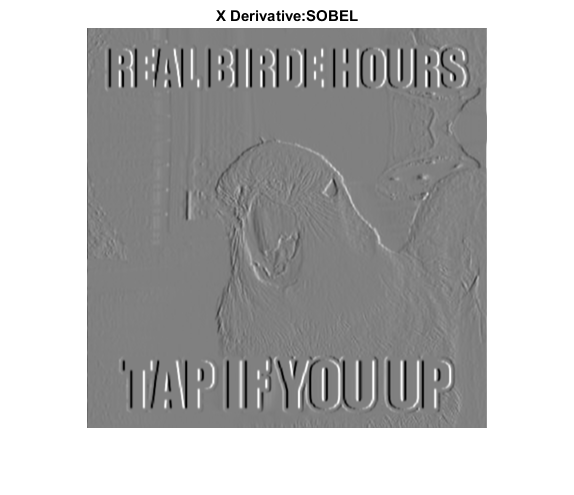
\includegraphics[width=1\linewidth]{img/sob1x}
		  \caption{X Derivative}
		  \label{fig:sobX}
	\end{subfigure}%
	\begin{subfigure}{.5\textwidth}
		  \centering
		  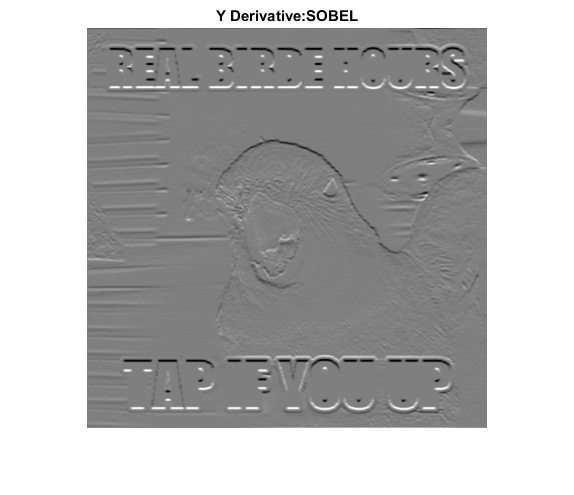
\includegraphics[width=1\linewidth]{img/sob2y}
		  \caption{Y Derivative}
		  \label{fig:sobY}
	\end{subfigure}
	\caption{Derivative Maps Using Sobel}
	\label{fig:sob1}
\end{figure}

\begin{figure}[h]
	\centering
	\begin{subfigure}{.5\textwidth}
		  \centering
		  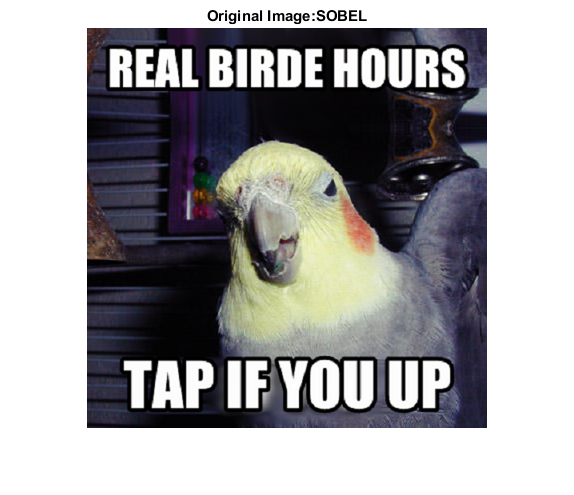
\includegraphics[width=1\linewidth]{img/sob0orig}
		  \caption{Original Image}
		  \label{fig:sobOrig}
	\end{subfigure}%
	\begin{subfigure}{.5\textwidth}
		  \centering
		  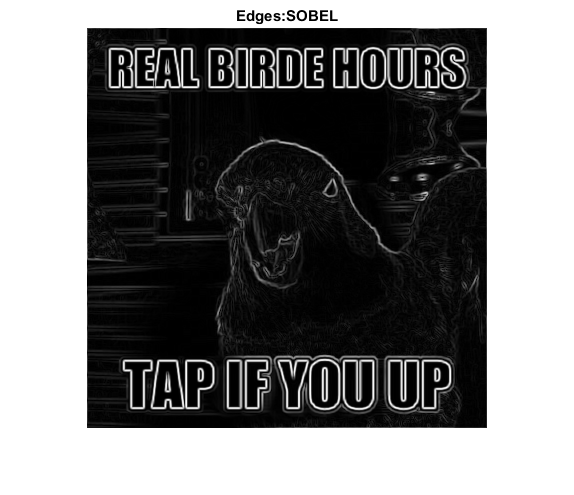
\includegraphics[width=1\linewidth]{img/sob3edge}
		  \caption{Edge Map}
		  \label{fig:sobEdge}
	\end{subfigure}
	\caption{Edge Detection Using Sobel}
	\label{fig:sob2}
\end{figure}
%%%%%%%%%%%%%%%%%%%%%%



\begin{figure}[h]
	\centering
	\begin{subfigure}{.5\textwidth}
		  \centering
		  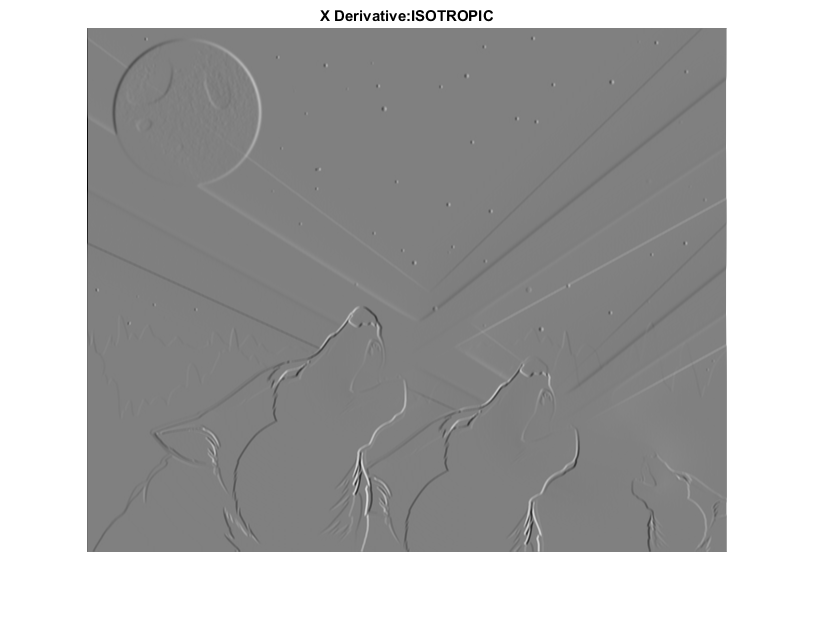
\includegraphics[width=1\linewidth]{img/iso1x}
		  \caption{X Derivative}
		  \label{fig:isoX}
	\end{subfigure}%
	\begin{subfigure}{.5\textwidth}
		  \centering
		  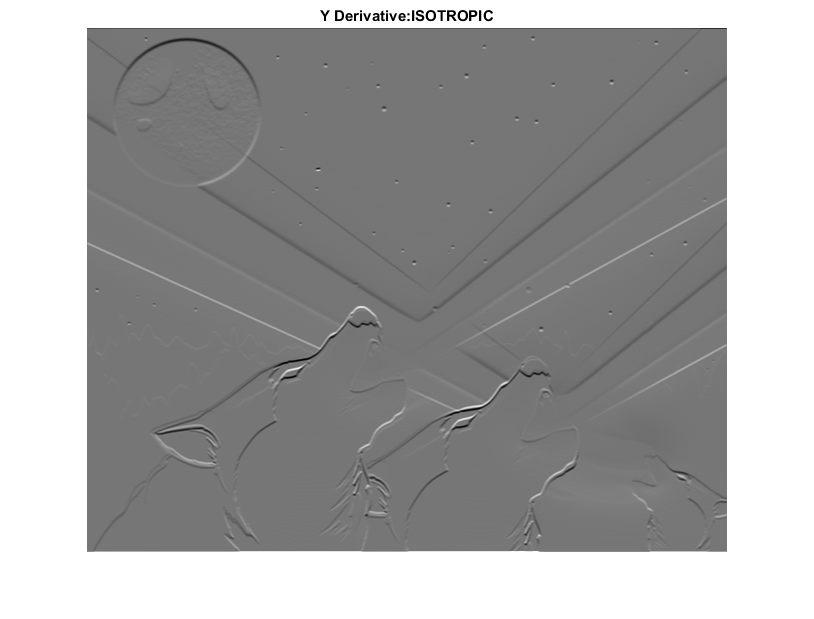
\includegraphics[width=1\linewidth]{img/iso2y}
		  \caption{Y Derivative}
		  \label{fig:isoY}
	\end{subfigure}
	\caption{Derivative Maps Using Isotropic}
	\label{fig:iso1}
\end{figure}

\begin{figure}[h]
	\centering
	\begin{subfigure}{.5\textwidth}
		  \centering
		  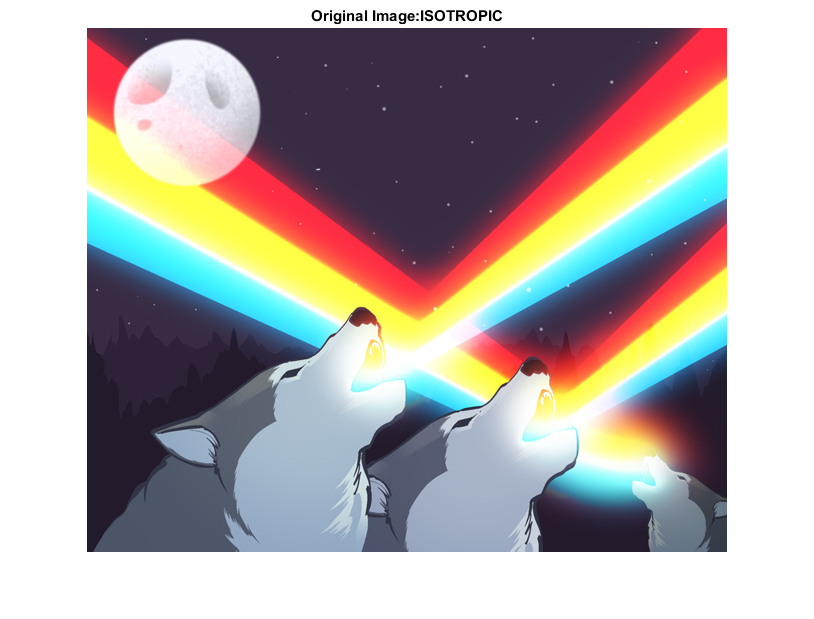
\includegraphics[width=1\linewidth]{img/iso0orig}
		  \caption{Original Image}
		  \label{fig:isoOrig}
	\end{subfigure}%
	\begin{subfigure}{.5\textwidth}
		  \centering
		  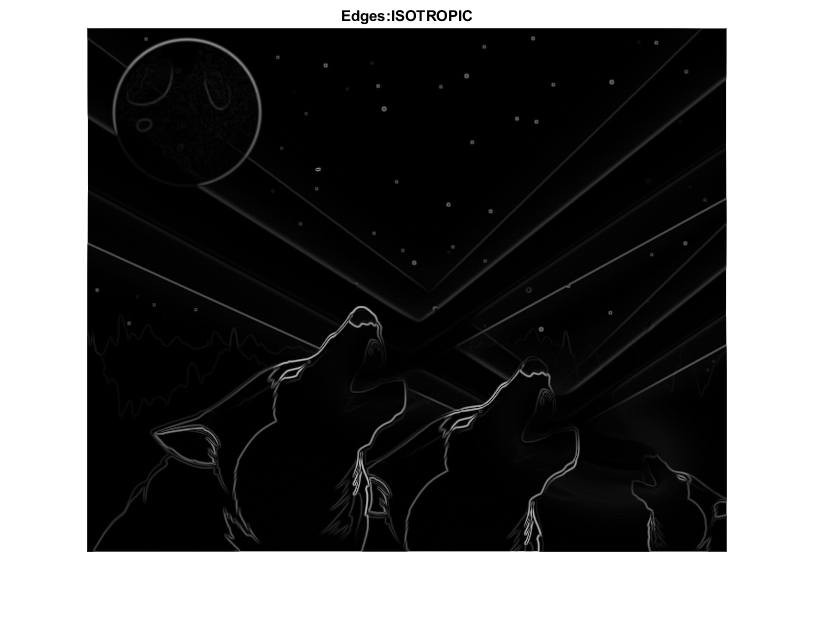
\includegraphics[width=1\linewidth]{img/iso3edge}
		  \caption{Edge Map}
		  \label{fig:isoEdge}
	\end{subfigure}
	\caption{Edge Detection Using Isotropic}
	\label{fig:iso2}
\end{figure}
%%%%%%%%%%%%%%%%%%%%%%


\begin{figure}[h]
	\centering
	\begin{subfigure}{.5\textwidth}
		  \centering
		  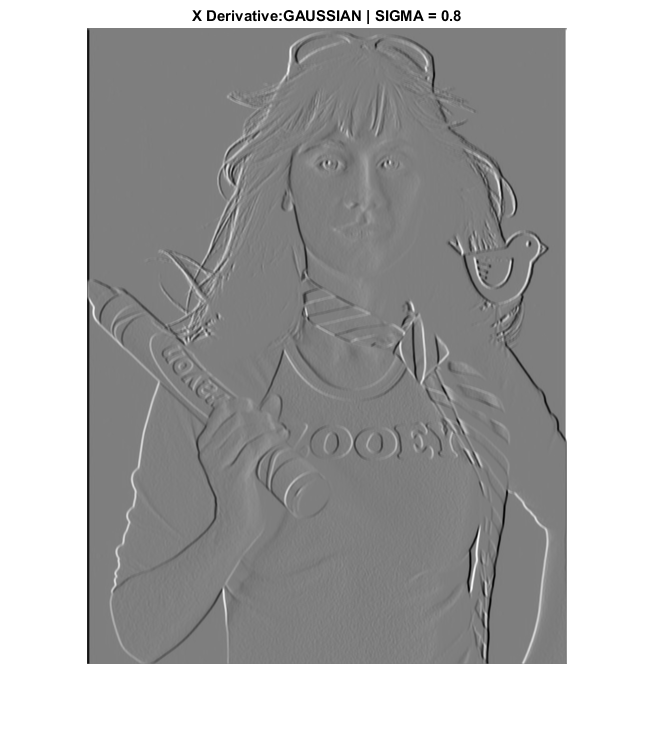
\includegraphics[width=1\linewidth]{img/gauss1x}
		  \caption{X Derivative}
		  \label{fig:gaussX}
	\end{subfigure}%
	\begin{subfigure}{.5\textwidth}
		  \centering
		  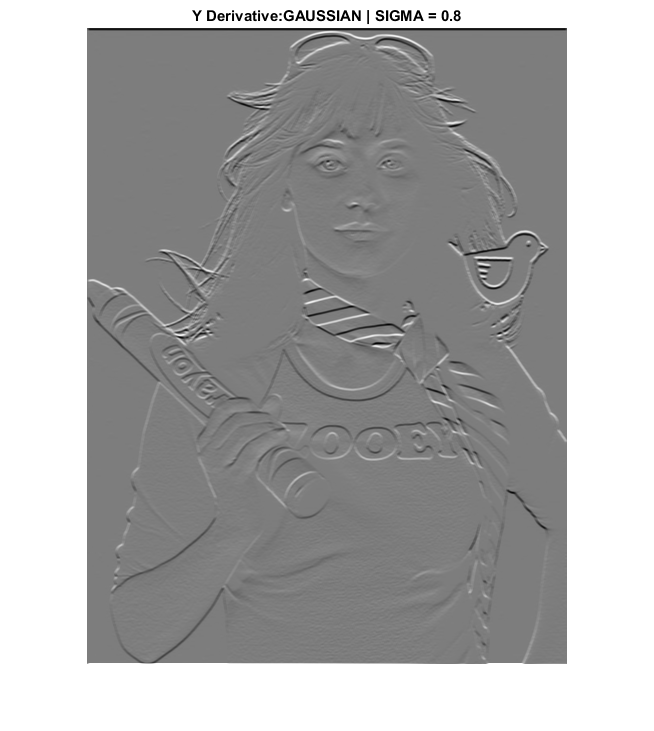
\includegraphics[width=1\linewidth]{img/gauss2y}
		  \caption{Y Derivative}
		  \label{fig:gaussY}
	\end{subfigure}
	\caption{Derivative Maps Using Gaussian}
	\label{fig:gauss1}
\end{figure}

\begin{figure}[h]
	\centering
	\begin{subfigure}{.5\textwidth}
		  \centering
		  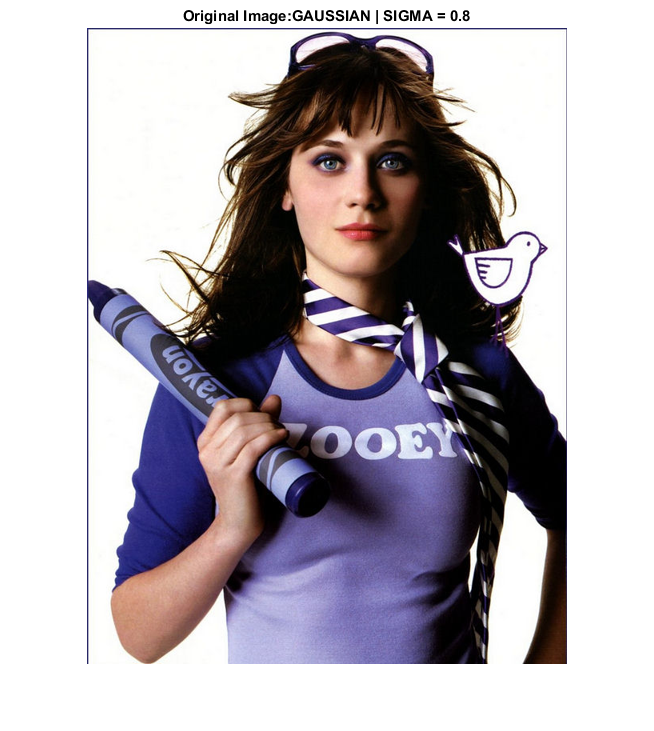
\includegraphics[width=1\linewidth]{img/gauss0orig}
		  \caption{Original Image}
		  \label{fig:gaussOrig}
	\end{subfigure}%
	\begin{subfigure}{.5\textwidth}
		  \centering
		  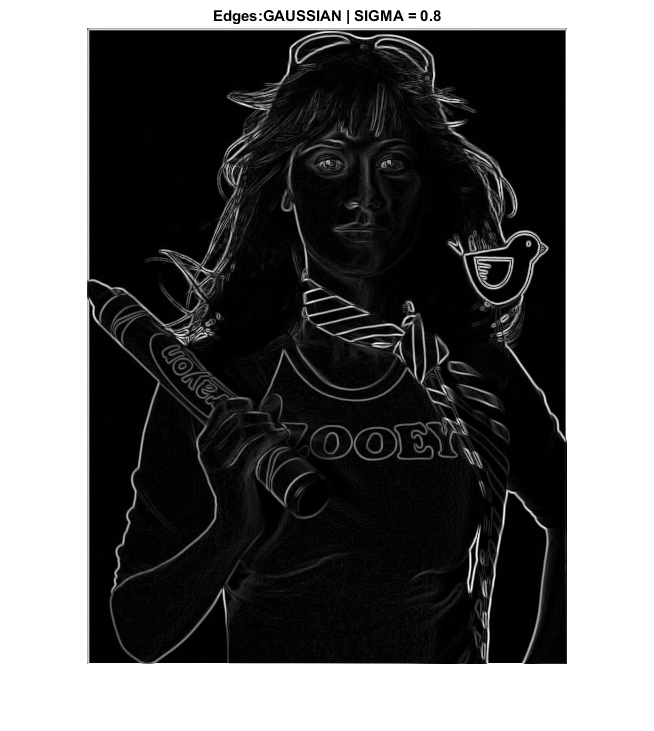
\includegraphics[width=1\linewidth]{img/gauss3edge}
		  \caption{Edge Map}
		  \label{fig:gaussEdge}
	\end{subfigure}
	\caption{Edge Detection Using Gaussian}
	\label{fig:gauss2}
\end{figure}









\lstset{language=Matlab,%
    %basicstyle=\color{red},
    breaklines=true,%
    morekeywords={matlab2tikz},
    keywordstyle=\color{blue},%
    morekeywords=[2]{1}, keywordstyle=[2]{\color{black}},
    identifierstyle=\color{black},%
    stringstyle=\color{mylilas},
    commentstyle=\color{mygreen},%
    showstringspaces=false,%without this there will be a symbol in the places where there is a space
    numbers=left,%
    numberstyle={\tiny \color{black}},% size of the numbers
    numbersep=9pt, % this defines how far the numbers are from the text
    emph=[1]{for,end,break},emphstyle=[1]\color{red}, %some words to emphasise
    %emph=[2]{word1,word2}, emphstyle=[2]{style},    
}

\clearpage
\begin{lstlisting}[caption = {Main Script}]
function edge()

    clc
    close all

    %Image Files
    f1 = 'angry.png';
    f2 = 'bike.jpg';
    f3 = 'real.png';
    f4 = 'wolf.jpg'; 
    f5 = 'zooey.jpg';
    
    %KERNEL methods
    rob = 'ROBERTS';
    pre = 'PREWITT';
    sob = 'SOBEL';
    iso = 'ISOTROPIC';
    gau = 'GAUSSIAN';
  
    %Convert each image to grayscale doubles
    %See prepimage() function below
    [ img01, img01g ] = prepimage( f1 );
    [ img02, img02g ] = prepimage( f2 );
    [ img03, img03g ] = prepimage( f3 );
    [ img04, img04g ] = prepimage( f4 );
    [ img05, img05g ] = prepimage( f5 );

    %Generate Kernels
    %See get_kernel() function below
    [ k01x, k01y ] = get_kernel(rob); 
    [ k02x, k02y ] = get_kernel(pre); 
    [ k03x, k03y ] = get_kernel(sob); 
    [ k04x, k04y ] = get_kernel(iso); 
    [ k05x, k05y ] = get_kernel(gau, 0.8 ); 

    %Generate Images (x derivative, y derivative, edge map)
    %See get_edge() function below
    [ map01x, map01y, edge01 ] = get_edge( img01g, k01x, k01y );
    [ map02x, map02y, edge02 ] = get_edge( img02g, k02x, k02y );
    [ map03x, map03y, edge03 ] = get_edge( img03g, k03x, k03y );
    [ map04x, map04y, edge04 ] = get_edge( img04g, k04x, k04y );
    [ map05x, map05y, edge05 ] = get_edge( img05g, k05x, k05y );

    %Display Images (original image, x derivative, y derivative, edge map)
    %see genfigure() function below
    genfigure( img01, map01x, map01y, edge01, rob);
    genfigure( img02, map02x, map02y, edge02, pre);
    genfigure( img03, map03x, map03y, edge03, sob);
    genfigure( img04, map04x, map04y, edge04, iso);
    genfigure( img05, map05x, map05y, edge05, strcat(gau, ' | SIGMA = 0.8'));

end
\end{lstlisting}

\clearpage

\begin{lstlisting}[caption = {Preparing Images}]
function [ img, img_g ] = prepimage( file )
    %Read in image, scale it down a bit, return colored img and grayscale
    img = imread( file );
    img = imresize( img, 0.8 );
    img_g = rgb2gray( img );
    img_g = double( img_g );
end
\end{lstlisting}


\begin{lstlisting}[caption = {Generate Figures}]

function genfigure( i, ix, iy, iedge, descr )

    %Generate Images (original image, x derivative, y derivative, edge map)
    set(gca,'LooseInset',get(gca,'TightInset'))

    %Show images with appropriate descriptions
    figure, imshow(i,[]);    
    title(strcat('Original Image: ', descr));
    
    figure, imshow(ix,[]);    
    title(strcat('X Derivative: ', descr));

    figure, imshow(iy,[]);
    title(strcat('Y Derivative: ', descr));

    figure, imshow(iedge,[]);
    title(strcat('Edges: ', descr));

end

\end{lstlisting}


\begin{lstlisting}[caption = {Generate Edge Map}]
function [ derX, derY, edge ] = get_edge( image, kernX, kernY )
    %Generate X Derivative Map through convolution
    derX = convolution( image, kernX );
    %Generate Y Derivative Map through convolution
    derY = convolution( image, kernY );
    %Generate Edge Map through gradient magnitude
    edge = sqrt(derX.^2 + derY.^2);
end
\end{lstlisting}

\clearpage

\begin{lstlisting}[caption = {Convolution}]
function [ G ] = convolution( scene, kernel )
    %%For Convolution, just Flip the filter in both directions
    %%Then apply Correlation as before...
    %%BTW rot90(x,2) is faster than flipud() + fliplr() which also works...
    kernel = rot90(kernel,2);
    
    %%Find the dimensions for the scene and kernel
    [kH, kW] = size(kernel);
    [sH, sW] = size(scene);

    %Get Half-Dimensions of Kernel to determine padding on each side
    kH2 = floor(kH / 2);
    kW2 = floor(kW / 2);

    %GENERATE HORIZONTAL PADDING
    pad = zeros(kH2,sW);
    %PAD TOP OF IMAGE
    scene = vertcat(pad,scene);
    %PAD BOTTOM OF IMAGE
    scene = vertcat(scene,pad);
    
    %GENERATE VERTICAL PADDING
    pad = zeros(sH + 2 * kH2,kW2);
    %PAD LEFT SIDE OF IMAGE
    scene = horzcat(pad,scene);
    %PAD RIGHT SIDE OF IMAGE
    scene = horzcat(scene,pad);


    %%set F, G, H matrices so that they match what's in the book.
    G = double(zeros(sH, sW));
    F = scene;
    H = kernel;

    %Calculate Correlation. Fixed so the summation appears closer to slides
    for i = 1:sH
        for j = 1:sW
        total = 0;
            for u = 1:kH
                for v = 1:kW
                    total = total + H(u,v) * F(i + u - 1,j + v - 1);
                end
            end
            G(i,j) = total / (sH * sW * kH * kW);
        end
    end
    
end
\end{lstlisting}

\clearpage

\begin{lstlisting}[caption = {Generate Kernel}]
function [ Gx, Gy ] = get_kernel( kType, kSigma )
    %Ensure first arg is always caps
    kType = upper(kType);
    %Only Gaussian has kSigma
    if nargin < 2
       kSigma = 0;
    end
    if strcmp( kType, 'ROBERTS')
        %ROBERTS:
        Gx = [  0  1  ;
               -1  0 ];
        Gy = [  1  0  ;
                0 -1 ];  
    else
        %HANDLE THE OTHERS
        if strcmp( kType, 'PREWITT')
            %PREWITT:
            p = 3;
        elseif strcmp( kType, 'SOBEL')
            %SOBEL:
            p = 4;
        elseif strcmp( kType, 'ISOTROPIC')
            %ISOTROPIC:
            p = 2 + sqrt(2);
        elseif strcmp( kType, 'GAUSSIAN')
            %GAUSSIAN:
            p =  2 * pi * ( kSigma * kSigma ) ;
        end
        
        if strcmp( kType, 'GAUSSIAN')
        %Gradient Kernel Family used for Gaussian:
        GradKernX = [   -1    0    1   ;
                        -1    0    1   ;
                        -1    0    1  ];
        GradKernY = [   -1   -1   -1   ;
                         0    0    0   ;
                         1    1    1  ];                     
        else
        %Gradient Kernel Family used for Prewitt, Sobel, Iso:
        GradKernX = [   -1    0    1   ;
                        2-p   0   p-2  ;
                        -1    0    1  ];
        GradKernY = [   -1   2-p  -1   ;
                         0    0    0   ;
                         1   p-2   1  ];            
        end

        %Apply finite difference kernels
        Gx = (1/p) * GradKernX;
        Gy = (1/p) * GradKernY;
    end
end
\end{lstlisting}


\end{homeworkProblem}
\clearpage

%----------------------------------------------------------------------------------------

\end{document}
